\documentclass[a4paper,12pt]{article}
\usepackage[english]{babel}
\usepackage{graphicx}
\usepackage{csvsimple}
\usepackage{pgfplotstable}
\usepackage{booktabs}
\usepackage{chngcntr}
\usepackage{sectsty}
\usepackage{pdfpages}
\usepackage{longtable}
\usepackage{tocloft}
\usepackage{amsmath}

%\usepackage[pdftex]{graphicx}
\usepackage[ansinew]{inputenc}
\usepackage{geometry}
%\usepackage{bbold}
\geometry{a4paper,left=2.5cm,right=2.5cm, top=2.5cm, bottom=3cm}
\newcommand{\HRule}{\rule{\linewidth}{0.5mm}}

\usepackage{textcomp}
\usepackage[hyphens,spaces]{url}

\begin{document}
\sloppy
\sectionfont{\LARGE}
\subsectionfont{\Large}
\subsubsectionfont{\Large}
\counterwithin{figure}{section}
\counterwithin{table}{section}

\begin{titlepage}


%%LR
\sffamily

\begin{center}


% Oberer Teil der Titelseite:

\includegraphics[width=0.3\textwidth]{../figures/LMU-logo.jpg}
\hfill

\includegraphics[width=0.4\textwidth]{../figures/TUM-logo.jpg}  
\\[5cm]

{\LARGE Department of Bioinformatics and Computational Biology}\\[0.5cm]
{Technische Universit\"at M\"unchen}\\
[2cm]
{\Large Master's Thesis in Bioinformatics}\\[1.5cm]

% Title
\HRule \\[0.4cm]
{ \huge \bfseries Variation of HERV elements in the KORA cohort
}\\[0.4cm]

\HRule \\[1.5cm]

{\Large Julian Schmidt}\\[2.5cm]

\vfill
\end{center}
\end{titlepage}
\pagestyle{empty}

%%LR comprehensive title
\begin{titlepage}
{\sffamily


\begin{center}

\includegraphics[width=0.3\textwidth]{../figures/LMU-logo.jpg}
\hfill

\includegraphics[width=0.4\textwidth]{../figures/TUM-logo.jpg}  
\\[1.5cm]  

{\LARGE Department of Bioinformatics and Computational Biology}\\[0.5cm]
{Technische Universit\"at M\"unchen}\\[1cm]

{\Large Master's Thesis in Bioinformatics}\\[2cm]
{\textbf{\LARGE Variation of HERV elements in the KORA cohort}}\\[2cm]
{\textbf{\LARGE Variation von HERV elementen in der KORA Kohorte}}\\[4cm]

\end{center}
\begin{center}\Large
  \begin{tabular}{ll}
    Author:& Julian Schmidt\\
    Supervisor: & Dr. Matthias Heinig\\
    Advisor:        & Johann Hawe\\
    Submitted:     &  15.04.2018\\
  \end{tabular}
\end{center}

}% end title page
\end{titlepage}

\pagenumbering{gobble}

\tableofcontents
\newpage

\pagestyle{plain}
\pagenumbering{arabic}
\section{Introduction}

\subsection{Epigenetics}
\begin{itemize}
\item central dogma of biology
\item rising importance of other factors atop DNA \textrightarrow epigenetics
\item quick overview epigenetic marks
\item chromatin states
\item DNA methylation 
\begin{itemize}
\item most understood and researched epigenetic mark \cite{Smith2013}
\item mechanism: methylation fifth position of cytosine, almost exclusively in CpG context in mammals, installed and maintained by 3 enzymes: DNA methyltransferase 1/3A/3B (DNMT1/...)
\item generally considered as silencing mark
\item CpG islands = groups of cg pairs, often in promoter regions, usually hypomethylated
\item promoter regions kept free of methylation
\end{itemize}
\item snp -> cpg -> expression pattern
\item TF <-> cpg interaction
\end{itemize}


\subsection{Human endogenous retroviruses}
When the draft for the first human genome was published in 2001\cite{Venter1304} there was the expectation, that it would allow to fully understand the human genome. But soon after genes were annotated less than 5\% of the genome was found to be protein coding\cite{Consortium2001} and later on the amount of exonic protein coding DNA was estimated to be as low as 1.2\%\cite{Encode2012}. The remaining majority of genome was often labeled as non-functional "junk DNA"\cite{Pennisi1159}. 

Since then this notion has generally been revoked. Especially within the two phases of the Encyclopedia of DNA Elements (ENCODE) project\cite{Encode2012}, participation in some functional role has been assigned to up 80.4\% of the human genome. 

% With the discovery of functional RNAs\cite{x}, ...\cite{x} and the ever growing knowledge about regulatory elements\cite{x} understanding and discovering the function of the DNA that doesn't directly code for proteins has been one of the biggest areas of interest. 

Still up to this day there are areas in the genome that are hard to analyze. Especially repetitive sequences cause huge problems for any method that relies on sequencing\cite{Treangen2011}. In human repetitive DNA makes up about 50\% of the whole Genome\cite{Treangen2011}. There are five major classes of repetitive elements: Satellites, short interspersed nuclear elements (SINE), long interspersed nuclear elements (LINE), DNA transposons and long terminal repeat (LTR) retrotransposons. 

In this work we focused on a subclass of the latter repeat class. Human endogenous retroviruses (HERVs) belong to the class of LTR retrotransposons and make up about 8\% of the human genome\cite{APM:APM12476}. HERVs originate from retroviruses that infected the germ line of humans or human ancestors up to 30 million years ago\cite{10.1146/annurev.genom.7.080505.115700}. Therefore, they became dormant in the genome and are inherited in a Mendelian fashion. Newly integrated endogenous retroviruses (ERVs) share the typical structure of the viruses they originate from. This means they contain at least the four main genes in the order $5'-gag-pro-pol-env-3'$. Gag encodes the matrix and capsid proteins. Pro codes for a protease. Pol is the reverse transcriptase and integrase and env codes for the surface proteins. Furthermore, they have two flanking LTRs that originate from a duplication of the sequence, where the retrovirus was integrated\cite{10.1146/annurev.genom.7.080505.115700}.   

However, endogenous retroviruses in human are generally not able to replicate. This is due to a high level of degeneration of the HERV gene sequences due to mutations and deletion introducing frame shifts as well as homologous recombination of the flanking LTRs leading elements containing only a single LTR and losing the entire coding body\cite{10.114610.1146/annurev.genom.7.080505.115700}. Additionally, the promoter activity of LTRs is commonly silenced by hypermethylation\cite{Smith2013}.

\begin{itemize}
\item tie in methylation -> silencing LTR promoter activity 
\item discovered roles of hervs in general regulation/diseases
\item 
\end{itemize}

\subsection{Effect network analysis}
\begin{itemize}
\item many bioinformatics methods find correlations, but not direct cause
\item attempt to discern direct connections from bigger data webs
\item hope to find possible biological mechanisms of gene regulation = path in model 
\item used approach: Gaussian Graphical models
\end{itemize}


\newpage
\section{Data}


\subsection{HERV annotation}
HERV annotation was pertained from RepeatMasker\cite{RepeatMasker} repeat library. RepeatMasker is a tool that screens DNA sequences against a library interspersed repeats and low complexity DNA sequences. It generates an annotation of identified repeats and masks them in the query sequence.

The track representing all identified elements from the RepeatMasker library for human genome hg19 was downloaded from the UCSC genome browser download section \url{(http://hgdownload.soe.ucsc.edu/goldenPath/hg19/database/rmsk.txt.gz)}. It contains a total of 5298130 occurrences of repeats. Each entry consists of 17 values. These are repeat name, the repeat class and family, as well as the chromosome, strand, and the genomic start and end position of the repeat occurrence. Furthermore it contains the area of the known repeat sequence, that is covered by the occurrence. It also contains the quality of the alignment of the repeat sequence to the annotated position using the Smith Waterman alignment score\cite{SMITH1981195} and the number of base mismatches, deletions and insertions per thousand base pairs. Finally, there is an indexing field used to speed up chromosome range queries and the first digit of the id field in the RepeatMasker output file. The first 10 lines of the track are shown in table \ref{tab:RepeatMaskerTrack}.

\begin{table}[b]
\centering
\label{tab:RepeatMaskerTrack}
\resizebox{\textwidth}{!}{
\pgfplotstabletypeset[
    col sep=tab, 
    header=true,    
	columns={bin, swScore, milliDiv, milliDel, milliIns, genoName, genoStart, genoEnd, genoLeft, strand, repName, repClass, repFamily, repStart, repEnd, repLeft, id},
	columns/genoName/.style={column type=l,string type},
	columns/strand/.style={column type=l,string type},
	columns/repName/.style={column type=l,string type, string replace*={_}{\textunderscore}},
	columns/repClass/.style={column type=l,string type, string replace*={_}{\textunderscore}},
	columns/repFamily/.style={column type=l,string type, string replace*={_}{\textunderscore}},
	every head row/.style={before row=\hline, after row=\hline},
	every last row/.style={after row=\hline}]{../tables/head.repeatmasker.track.tsv}}
\caption{First ten rows of the RepeatMasker annotation on hg19}
\end{table}

To extract HERV elements the annotation was filtered on different columns generating three sets of variable size. Multiple HERV sets were created as an attempt to cover different possible definitions of HERV elements.

This work only discerned between different HERV element types by defining different HERV sets. Therefore, within each set annotations, whose genomic positions overlap or are directly adjacent, were merged into one element.

A first set, HERV set 1 (HERV S1) was constructed by extracting all elements that contained "ERV" in the repeat name column. This set
The resulting 42508 annotations condensed to 35358 elements after merging. The elements have a mean width of 956 bp and cover a total of 33.8 Mbp, which is about 1.04\% of the human genome. The distribution of element lengths in HERV S1 is shown in Figure \ref{fig:hervS1.lengths.hist}  

Alternatively, filtering the annotation for "ERV" in the super family column leads to 696689 annotations. HERV set 2 (HERV S2) contains all endogenous retroviral sequences found in the human genome. Therefore, it is the most comprehensive set and it is the focus of detailed results that are shown and discussed. After merging overlapping and adjacent annotations this led to 612594 elements. Their mean width is 430 bp and they make up to 263.4 Mbp or ca 8.13\% of the human genome. 

A third set "HERV set 3" (HERV S3) was constructed by filtering the repeat name column for "HERV", which resulted in 21361 annotations. As this set contains only elements that are explicitly named "HERV", we expect it to contain elements, that were inserted directly into the human genome. Merging overlapping and adjacent annotations resulted in 15284 elements with an average width of 1480 bp and a combined length of 22.6 Mbp.

\begin{figure}[tb]
	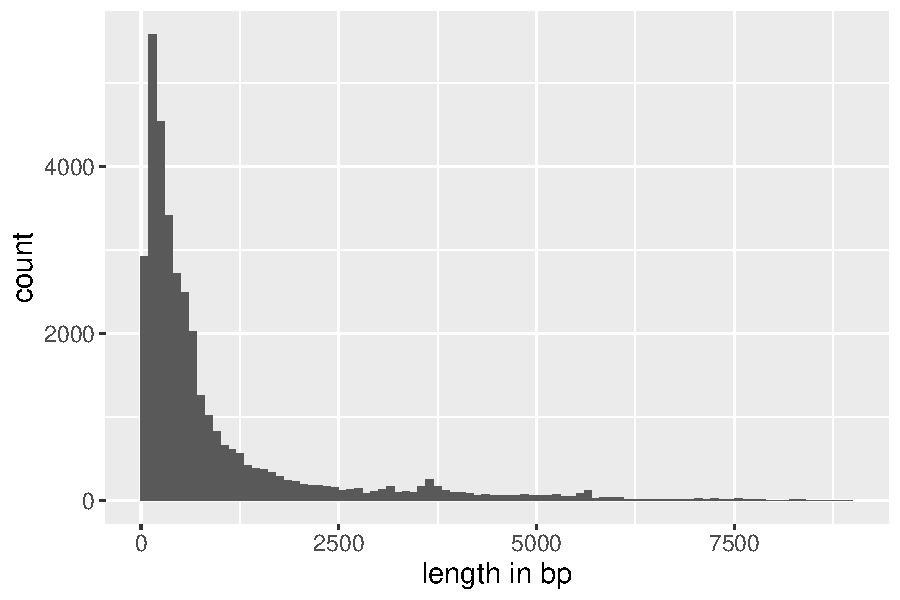
\includegraphics[scale = 1, keepaspectratio = true]{../figures/hervS1_lengths_hist}  
	\caption{Length distribution of elements in HERV S2"}
    \label{fig:hervS1.lengths.hist}
\end{figure}


\subsection{KORA}
The functional data for our analysis of gene regulatory mechanisms are made up up expression, methylation and genotype data. These were collected in the light of the platform for Cooperative Health Research in the Region of Augsburg, short KORA. It contains health surveys as well as examinations of individuals of German nationality living in the area of Augsburg, Bavaria.
The objective of KORA is to track changes in health conditions over a long period in order to identify and examine the causes, effects and development of chronical diseases.

The data used in this work originates from the KORA F4 Survey, which was conducted from 2006 to 2008 and comprised samples of 3080 individuals. Of these data was available for 3020 individuals. F4 is a follow up study to the KORA S4 Survey performed from 1999 to 2001. It contains 4261 individuals. 

All measurements were performed on whole blood samples. Houseman blood counts\cite{10.3389/fgene.2016.00023} describing the composition of different cell types for each individual had previously been calculated from the methylation data. They were used to weight certain cell type specific data. 

Not all essays are available for all samples. Therefore different analyses were performed on varying sets of individuals according to availability of the required data types. A diagram of the samples available for each essay can be seen in figure \ref{fig:samples.venn}. 

\begin{figure}[tb]
\begin{center}
	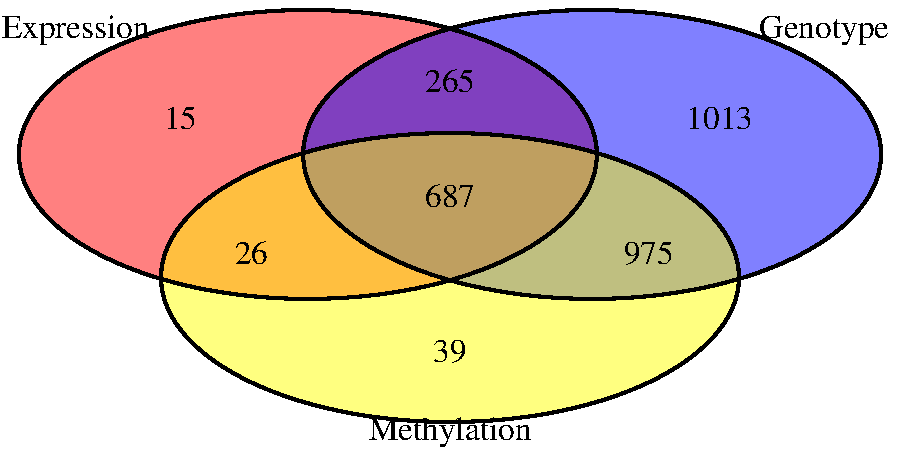
\includegraphics[scale = 1, keepaspectratio = true]{../figures/samples_venn}  
	\caption{Number of samples with genotype, expression and methylation measurements in KORA F4 Survey}
    \label{fig:samples.venn}
\end{center}
\end{figure}

\subsubsection{Expression}
The expression data was generated using the HumanHT-12 v3.0 Gene Expression BeadChip. The chip can measure expression values for 49576 probes. However, only 47864 probes represent an actual genomic location. The remaining probes are control probes used to assess the quality of the measurements and infer the background for measurements. 

Measurements for 993 individuals are available from the KORA F4 survey. The comprise values for a total of 48803 probes per sample. Probes that do not map to a genomic location were excluded in all analyses, leaving 47864 probes. Of these 29521 are annotated to a total of 19288 genes. 

The available data had already been quantile normalized, corrected for the background and log-transformed. 

Figure \ref{fig:expr.raw.hist.cov} shows the distribution and coefficient of variation over all probes and samples. Apart from a tail of some probes with very high expression values figure \ref{fig:expr.raw.hist.cov}A roughly resembles a standard distribution. 

\begin{figure}[tb]
	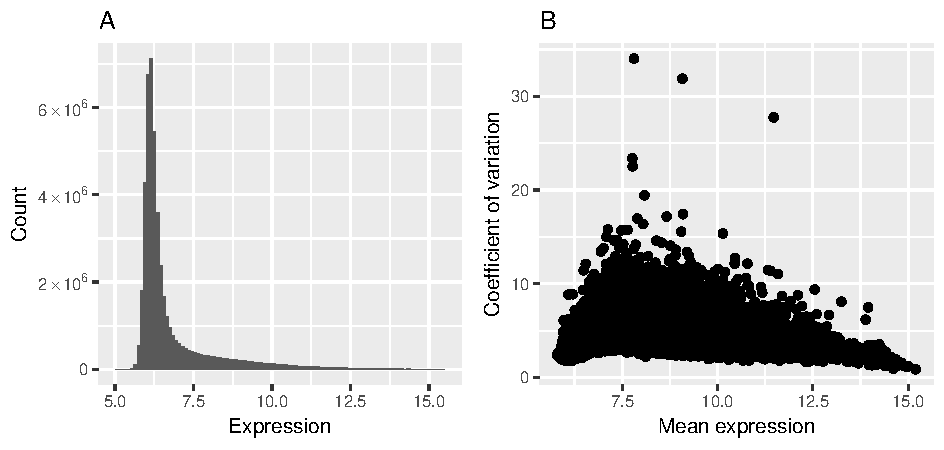
\includegraphics[scale = 1, keepaspectratio = true]{../figures/expr_raw_hist_cov}  
	\caption{Distribution of expression values (A) and coefficient of expression variation (B) of 47864 probes in 993 individuals.}
    \label{fig:expr.raw.hist.cov}
\end{figure}


Probes that could not be mapped to genes were not discarded to avoid losing data for HERV regions, which are only sparsely annotated with genes and were the focus of this work and. Therefore, most analyses were performed on probe level or a mix of probes and genes.


\subsubsection{Methylation}
DNA methylation was measured using the Infinium HumanMethylation450K BeadChip, which interrogates methylation levels at 485577 genomic locations. Methylation intensities had already been corrected and transformed to beta values. Beta values have a range from 0 to 1 and represent the fraction of copies of a CpG site that are methylated in a sample.

No imputation of missing measurements was performed for the methylation data. Therefore, only 44335 probes have measurements in all samples available. Overall there are about 11.2 million missing values, which makes up 1.3\% of all measurements and on average 23 samples missing per probe. 

Methylation data was available for 1727 individuals and 485512 sites, which make up all 'cg' and 'ch' probe type probes. The distribution of beta values and the variances over all samples and probes is shown in figure \ref{fig:meth.raw.hist.var}. As seen in figure \ref{fig:meth.raw.hist.var}A, the interrogated CpG sites tend to be either entirely methylated or unmetylated within single samples. However, as B shows there is some variance between individuals in most CpG-sites. The low variance for very low and very high betas is explained by the fact that for a CpG site to have a mean close to 0 all samples have to have a value close to 0. Therefore, the variance also is very low.

 
\begin{figure}[tb]
	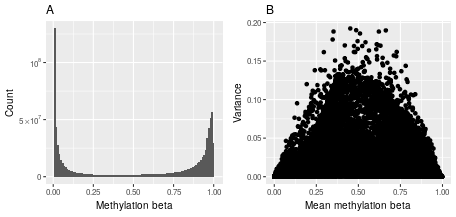
\includegraphics[scale = 1, keepaspectratio = true]{../figures/meth_raw_hist_var}  
	\caption{Distribution of all methylation beta values (A) and variance (B) of 485577 CpGs between 1727 individuals.}
    \label{fig:meth.raw.hist.var}
\end{figure}

 
\subsubsection{Genotypes}
Genotyping was performed with the Affymetrix Axiom array. On the data set used in this work genotypes had already been called using the Iluminus calling algorithm and missing values had been imputed using the IMPUTE2 software\cite{10.1371/journal.pgen.1000529}. Furthermore, imputation results had already been filtered at IMPUTE value of 0.4.  

%TODO rewrite
Additionally SNPs with a minor allele frequency of less than one percent had been removed, which allows used association analyses to be have more powerful test statistics.

In total measurements of 9533127 SNPs for 2940 individuals were available in the form of continuous values from 0 to 2 with 0 representing no occurrence of the SNP and 2 meaning the SNP is present in both chromosomes. Non integer values mean that different genotypes were measured in different cells in the sample and the resulting value describes the fraction of the occurrence of the variant. 

\subsubsection{Covariates}
Several covariates were known for each sample. They were used to correct expression and methylation values for common effects. 

%TODO which sex is which?
The sex of all participants was known. Of the 3020 participants with any available data 1458 were SEX1 and the remaining 1562 were SEX2. The 697 individuals that had all three essays available contained 348 men/women and 339 women/men.
Further covariates specific to participating individuals are sex, age, body mass index (BMI) and white blood cell count. An overview of these covariate values for all 3020 individuals and the individuals with all three essays available is shown in table \ref{tab:covariate.overview}.


%TODO fix tables, add caption
\begin{table}[h!]
  	\begin{minipage}{.45\textwidth}
    \pgfplotstabletypeset[
    col sep=tab, 
    header=true,    
	columns={Covariate, Minimum, Maximum, Mean},
	columns/Covariate/.style={column type=l,string type},
	every head row/.style={before row=\hline, after row=\hline},
	every last row/.style={after row=\hline}]{../tables/full.covariate.overview.tsv}
    \end{minipage}
    \hfill
     \begin{minipage}{.45\linewidth}
    \pgfplotstabletypeset[
    col sep=tab, 
    header=true,    
	columns={Covariate, Minimum, Maximum, Mean},
	columns/Covariate/.style={column type=l,string type},
	every head row/.style={before row=\hline, after row=\hline},
	every last row/.style={after row=\hline}]{../tables/select.covariate.overview.tsv}
    \end{minipage}%
    \caption{Covariate overview}
	\label{tab:covariate.overview}
\end{table}

Finally, two experimental factors for the expression measurements, storage time and RNA integrity number (RIN) and plate, were known.

\subsubsection{Methylation quantitative trait loci}
Genotypic variants are known to effect methylation patterns in humans \cite{}. Therefore, we used previously processed methylation quantitative trait loci (meQTL) data to explore the mechanism of trans acting SNP-CpG associations. Associated pairs were used as a seed for trans-acting interaction networks.

For meQTLs a stringent definition of trans effects was used: A SNP-CpG pair was called a trans-meQTL only if they are located on different chromosomes. This definition differs from the one used for eQTM and eQTL calculation as described later. 

The data set contained a total of 11165559 significantly associated SNP-CpG pairs. 
70709 distinct CpG-sites and 2709428 SNPs were part of at least one meQTL. Of these 467915 pairs consisting of 3592 CpG-sites and 200761 SNPs were between different chromosomes. 


\subsection{Transcription factor binding}
DNA methylation plays a major role in the specifics of transcription factor binding sites\cite{Yineaaj2239}. We used transcription factor binding sites obtained from two publicly available sources to enrich information about CpG-sites of interest with transcription factors that bind nearby: 

The first source was the third version of the track "Transcription Factor ChIP-seq (161 factors) from ENCODE with Factorbook Motifs"\cite{10.1101/gr.139105.112} downloaded from the UCSC genome browser download section (\url{http://hgdownload.cse.ucsc.edu/goldenPath/hg19/encodeDCC/wgEncodeRegTfbsClustered/wgEncodeRegTfbsClusteredWithCellsV3.bed.gz}).

It combines 690 high quality ENCODE ChIP-seq data sets, which were processed with the Factorbook motif discovery and annotation pipeline\cite{10.1101/gr.139105.112}. The pipeline uses the tools MEME-ChIP\cite{10.1093/bioinformatics/btr189} and FIMO\cite{10.1093/bioinformatics/btr064} from the MEME software suite and merges discovered motifs with known motifs from Jaspar\cite{10.1093/nar/gkx1126} and TransFac\cite{10.1093/nar/gkj143} using machine learning methods and manual curation. 

The track contains a total of 438044 distinct peaks for 161 transcription factors in 91 cell types. For our analyses we filtered and combined the peaks for 23 blood related cell types. This leaves a total of 2173371 peaks for 125 transcription factors.  

The second source was the ReMap project\cite{10.1093/nar/gku1280}. It combines 395 publicly available ChIP-seq data sets covering 132 different transcription factors across 83 cell lines. ReMap uses Bowtie2\cite{} to map reads to the human genome and the tool MACS\cite{} for peak calling. The final data set was downloaded from the ReMap website\url{(http://tagc.univ-mrs.fr/remap/download/All/filPeaks_public.bed.gz)}.

There were a total of xxxxxx peaks for xxx transcription factors in the data set. After filtering for 19 blood related cell types xxxx peaks and xxx different transcription factors remained.  
%TODO fill in numbers when storage available 

Combining both filtered data sets lead to a total of 3847561 peaks of 145 different transcription factors.


\subsection{Chromatin states}
%TODO rewrite somewhat - but not used right now
Chromatin state annotations were downloaded from Roadmap Epgenomics Core 15-state model (\url{http://egg2.wustl.edu/roadmap/data/byFileType/chromhmmSegmentations/ChmmModels/coreMarks/jointModel/final}). The Model provides a whole genome chromatin state annotation of 200 bp wide windows to the following 15 states: Active Transcription Start Site (TSS), Flanking Active TSS, Transcription at gene 5' and 4', Strong transcription, Weak transcription, Genic enhancers, Enhancers, ZNF genes \& repeats, Heterochromatin, Bivalent/Poised TSS, Flanking Bivalent TSS/Enhancer, Bivalent Enhancer, Repressed PolyComb, Weak Repressed PolyComb and Quiescent/Low. The model is available for 127 diverse cell lines. 

It was generated using ChromHMM v1.10\cite{10.1038/nmeth.1906} on the chromatin marks H3K4me1, H3K4me3, H3K27me3, H3K9me3, and H3K36me3. ChromHMM is based on a multivarate Hidden Markov Model. 

In this work the annotations for 27 blood related cell lines were used. When combining the annotation for a genomic location of interest like a HERV element or a SNP, houseman blood counts were used to account of the cell composition of the whole blood samples. 


\newpage
\section{Methods}
Most computations were done using the statistical computing environment and programing language R, version 3.4.1\cite{Rlanguage}. Pre filtering steps on large files, that could not be loaded into random access memory, were performed using the bash command "awk", which runs scripts written in the "AWK" programming language.

\subsection{Overlaps}
The main objective of this thesis was to analyze the effects of HERV elements on the regulation of cell activity. 

To identify functional features like expression probes, genes, SNPs and CpG-sites that were associated with HERV elements, overlaps between these features and elements were calculated. Features were considered to be of interest for the analysis of an HERV element, if they overlapped by at least one base pair.

The calculation was performed using the function "findOverlaps" from the Bioconductor package "GenomicRanges"\cite{10.1371/journal.pcbi.1003118}. The function allows to identify overlaps between "GRanges" objects. These were constructed from BED files for all HERV sets as well as SNPs and retrieved from the Bioconductor packages available for analyses on the expression and methylation essays, "illuminaHumanv3.db"\cite{illuminaHumanv3.db} and "FDb.InfiniumMethylation.hg19"\cite{FDb.InfiniumMethylation.hg19} respectively.

The search for overlapping features was also performed on "GRanges" objects including all HERV elements as well as the 1kb or 2kb flanking regions of all elements. This was done to include functional features, that while not directly within HERV regions, are still likely to be influenced by them. Furthermore, this analysis was performed on all three HERV sets.

\subsection{Data normalization}
Before expression and methylation values were used for analyses, they were corrected for batch effects. For this we used the available covariates to calculate a linear models and regress out the respective residuals. The model used for expression values is shown in equation \ref{eq:expr.res.model} and considers the covariates age, sex, RNA integrity number (RIN), plate and storage time. The model for methylation values, shown in equation \ref{eq:meth.res.model},
includes the cell composition for the five blood cell types known from the houseman blood counts, as well as the first 20 principal components of the Illumina 450k array control-probes. 
\begin{equation}
\label{eq:expr.res.model}
Expr \sim 1+age+sex+RIN+plate+storage.time
\end{equation}
\begin{equation}
\label{eq:meth.res.model}
Meth \sim 1+CD4T+CD8T+NK+Bcell+Mono+\sum_{i=1}^{20} PC_{i}
\end{equation}


\subsection{eQTL/eQTM calculation}
As a preliminary analysis to interrogate the effect of genotype and methylation variants on expression, expression quantitative trait loci (eQTL) and expression quantitative trait methylation (eQTM) were calculated.

Calculations were performed using the Bioconductor package MatrixEQTL\cite{10.1093/bioinformatics/bts163}. MatrixEQTL tests for association of SNP-transcript pairs.  

We set the parameter \texttt{useModel = modelLINEAR}, which leads to the use of an  additive linear model. The association is modeled as simple linear regression and the absolute value of the sample correlation is used as test statistic.

After calculating the test statistics the p-values for all pairs that pass a defined significance threshold are calculated. These are corrected multiple testing using a Benjamini-Hochberg procedure\cite{10.2307/2346101}, adapted for not recording all p-values, as shown in equation \ref{eq:matrix.eqtl.transformation}

MatrixEQTL is rather efficient because it manages to reduce the calculation of the sample correlation over all SNPs and transcripts to one single large matrix multiplication. This is achieved by transforming the genotype and transcription values. 

MatrixEQTL also allows to include covariates in the QTL calculation. As the expression and methylation values used are residuals and therefore already corrected this option is not used. Furthermore, MatrixEQTL can differentiate between cis- and trans-interactions based on distance. The maximal distance to consider a pair on the same chromosome as cis was set to 500 kb. 
%TODO motivate cis-distance

The threshold for significant cis-QTLs during calculation was set to 10e-6 and 10e-8 for trans.



\subsection{Functional Analysis of Gene Sets}
In multiple analyses functional Gene Ontology enrichments were performed.

First a set of all GO annotations with any evidence code for gene symbols  was retrieved from the Bioconductor package AnnotationDbi\cite{AnnotationDbi}. 

Then a hypergeometric test\cite{GOstats} for overreprensentation is performed on a set of genes of interest. For most enrichments a custom background set of genes specific to the analysis is given. Finally, the p-values for overrepresented GO terms were adjusted for multiple testing using the Holm method\cite{10.2307/4615733}. Terms with an adjusted p-value of less than 0.05 were considered significantly overrepresented. 

\subsection{Gaussian Graphical Models}
%TODO write this stuff



\newpage
\section{Results}
\subsection{Normalized Data}
The distribution of the quantile normalized expression values and the expression residuals over all probes and samples can be seen in figure \ref{fig:expr.raw.res}. As expected the residuals follow a normal distribution. This is important for the calculation of the Gaussian graphical models, as the normal distribution of the data is one of base assumptions\cite{}.

\subsection{HERV region features}
In this section I will describe the expression probes that overlap with any HERV element and the cpgs and SNPs that lie within any HERV element and/or their flanking regions. The results for the set of all endogenous retroviral elements, HERV set 2, without flanking regions are described in detail. The results for the other sets and including flanking regions will be shown in tables or in the supplementary data.

\subsubsection{Expression}
A total of 2343 expression probes overlap directly with at least one of 2271 HERV elements from HERV S2. This means ca 4.50\% of all expression probes overlap with HERV elements and expression measurements are known for parts of ca 0.37\% of all HERV elements.

The mean expression of the probes overlapping with HERV elements, as shown in figure \ref{fig:hervS2.expr.var} is on average lower than for all probes (figure \ref{fig:expr.raw.hist.cov}A). The coefficient of variance, however, shows a very similar pattern for the whole set of probes and the considered subset.

\begin{figure}[tb]
	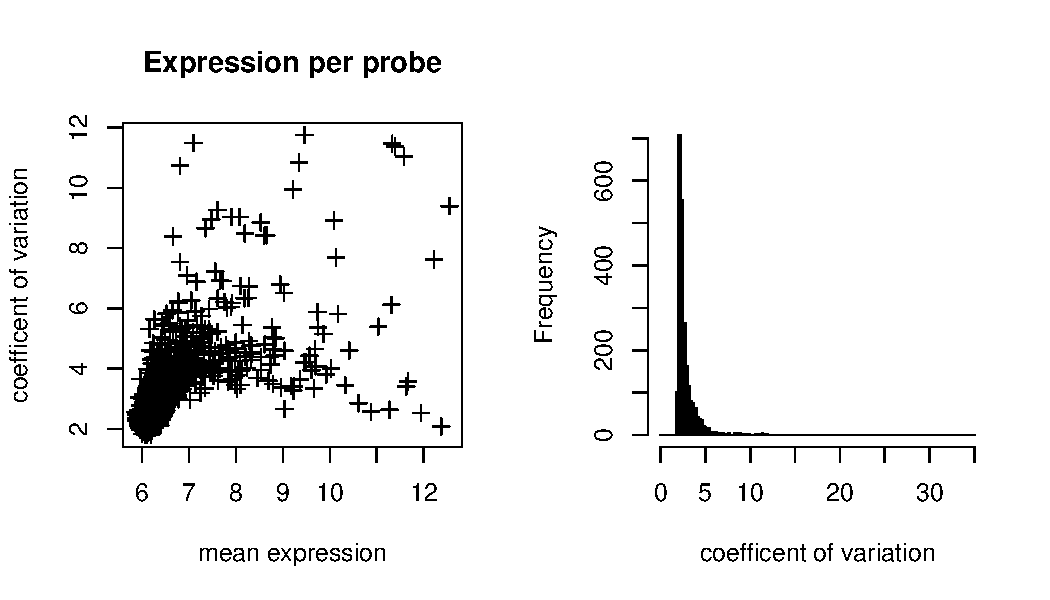
\includegraphics[scale = 1, keepaspectratio = true]{../figures/hervS2_expr_var}  
	\caption{Coefficient of expression variance over 993 individuals and 2343 expression probes overlapping with HERV S2.}
    \label{fig:hervS2.expr.var}
\end{figure}

Of these 2343 probes 510 were annotated to one of 449 different genes. I performed a GO enrichment for the biological process ontology on these genes with the set of all genes with available expression data as background. After correcting for multiple testing only the term defense response (GO:0006952, p-value=1.37e-5, fdr=0.047) was significantly enriched.

However, when including the 2kb flanking regions of HERV S2 and performing the GO enrichment on the 5518 identified genes, the six GO terms shown in table \ref{tab:hervS2.2kb.enrichment} are significantly overrepresented. They are all connected to defense response, especially against viruses.

\begin{table}[h!]
  \begin{center}
  \resizebox{\textwidth}{!}{
    \pgfplotstabletypeset[
    col sep=tab, 
    header=true,    
	columns={Term ID, Term, p, fdr},
	columns/Term ID/.style={column type=l,string type},
	columns/Term/.style={column type=l,string type},
	every head row/.style={before row=\hline, after row=\hline},
	every last row/.style={after row=\hline}]
    {../tables/hervS2.2kb.expr.enrichment.tsv}}
  \end{center}        
	\caption{Significantly enriched GO biological process terms among genes overlapping with HERV S2.}
	\label{tab:hervS2.expr.overlap.counts}
\end{table}
%Wrong hervS2.2kb


The results for all HERV sets and including flanking regions is shown in table \ref{tab:expr.overlap.counts}.

\begin{table}[h!]
  \begin{center}
    \pgfplotstabletypeset[
    col sep=tab, 
    header=true,    
	columns={Set,S1,S1.1kb,S1.2kb,S2,S2.1kb,S2.2kb,S3,S3.1kb,S3.2kb},
	columns/Set/.style={column type=l,string type},
	every head row/.style={before row=\hline, after row=\hline},
	every last row/.style={after row=\hline}]
    {../tables/expr.overlap.overview.tsv}
  \end{center}        
	\caption{Number of expression probes overlapping with different HERV sets and flanking regions. "Pairs" is the total number of overlaps occurring, "HERVs" is the number of distinct HERV elements that have an overlap with any of the expression probes, Probes describes the number of distinct expression probes that overlap with the HERV elements or their flanking regions, "Genes" is the number of distinct Genes that are annotated to these probes.}
	\label{tab:expr.overlap.counts}
\end{table}

\subsubsection{Methylation}
17077 CpG sites, equaling 3.52\% of all measured CpGs, were found within HERV S2 and 12871 distinct HERV elements (2.10\%) contain at least one interrogated CpG site.

CpGs associated with HERV S2, as shown in figure \ref{fig:meth.hervS2.hist.var}, tend to be highly methylated. The variance also is...

The number of CpG sites within all HERV sets and including flanking regions is shown in table \ref{tab:meth.overlap.counts}

\begin{table}[h!]
  \begin{center}
    \resizebox{\textwidth}{!}{
    \pgfplotstabletypeset[
    col sep=tab, 
    header=true,    
	columns={Set,S1,S1.1kb,S1.2kb,S2,S2.1kb,S2.2kb,S3,S3.1kb,S3.2kb},
	columns/Set/.style={column type=l,string type},
	every head row/.style={before row=\hline, after row=\hline},
	every last row/.style={after row=\hline}]
    {../tables/meth.overlap.overview.tsv}}
  \end{center}        
	\caption{Number of CpGs overlapping with different HERV sets and flanking regions. "Pairs" is the total number of overlaps occurring, "HERVs" is the number of distinct HERV elements that have an overlap with any of the expression probes, "CpGs" is the number of distinct CpG sites that lie within the HERV elements or their flanking regions.}
	\label{tab:meth.overlap.counts}
\end{table} 
\subsubsection{Genotypes}
A total of 890780 the considered SNPs are located within elements of HERV S2. This constitutes 9.34\% of all SNPs. These SNPs are found in 330744 distinct HERV elements. Therefore, 53.99\% contain at least one SNP.

The results for all sets and flanking regions are shown in table \ref{tab:snp.overlap.counts}

\begin{table}[h!]
  \begin{center}
    \resizebox{\textwidth}{!}{
    \pgfplotstabletypeset[
    col sep=tab, 
    header=true,    
	columns={Set,S1,S1.1kb,S1.2kb,S2,S2.1kb,S2.2kb,S3,S3.1kb,S3.2kb},
	columns/Set/.style={column type=l,string type},
	every head row/.style={before row=\hline, after row=\hline},
	every last row/.style={after row=\hline}]
    {../tables/snp.overlap.overview.tsv}}
  \end{center}        
	\caption{Number of SNPs overlapping with different HERV sets and flanking regions. "Pairs" is the total number of overlaps occurring, "HERVs" is the number of distinct HERV elements that have an overlap with any of the expression probes, "SNPs" is the number of distinct considered SNPs that lie within the HERV elements or their flanking regions.}
	\label{tab:snp.overlap.counts}
\end{table} 

\subsubsection{Chromatin states}
Data in /storage/groups/groups\textunderscore epigenreg/users/julian.schmidt ...

\subsection{eQTLs}
Associations were calculated for 156.4 millions cis acting SNP-expression probe pairs and 456.1 billion possible pairs in trans. 

812147 of cis-pairs were significantly associated with p-values of $1e-6$ or less. These significant eQTLs have a false discovery rate of less than $1.93e-4$. A total of 551728 distinct SNPs and 4903 expression probes were part of at least one cis-eQTL. 4145 of these probes are annotated to 3552 different genes. The remaining 
758 can not be assigned to a specific gene.

There were a total of 1511235 significant trans-eQTL with an p-value of less than 1e-8 and a FDR of less than $3.02e-4$. These are made up by 229332 distinct SNPs and 21338 expression probes. 11505 of the probes found in at least one trans-eQTL are annotated to 9389 different genes, while 9767 probes are not assigned to a gene.

In a previous work Schramm et al. \cite{10.1371/journal.pone.0093844} calculated eQTLs on expression and genotype data from 890 KORA F4 samples. They found significant cis-eQTLs for 4116 probes and considered only the pair of the most strongly associated SNPs with the probe. Of these pairs 2680 were also found in my analysis. 

Figure \ref{fig:global.eqtl.heatmap}A shows the fraction of significant to all possible  SNP-expression probe pairs, mapped to 10 Mpb windows. As expected the values at the diagonal are comparatively higher, containing all cis-eQTLs. 

The signatures of wildtype, heterogenous and homogenous mutated SNP site for the two eQTLs with the best and worst p-values in cis and trans are shown in figure \ref{fig:best.worst.eqtl.boxplot}. All eQTLs show clear differences in expression between different genotypic variants. 

45862 of the SNPs and 166 of the expression probes found in at least one cis-eQTL are located within HERV S2. When considering all significant associations, where either the SNP or the expression probe lie within a HERV element, a total of 112604 pairs remain. There are 5855 cis-eQTLs constituting one of 4748 SNPs within a HERV element controlling one of 128 expression probes, that overlap with a HERV element. 

When limiting trans-eQTLs to the ones that contain a HERV S2 SNP (23396) and/or expression probe (1227), 240301 remain. In 9177 of these pairs both are HERV related. 

The fraction of HERV S2 related SNP-expression probe pairs that proved to be significantly associated is shown in figure \ref{fig:global.eqtl.heatmap}B. The distribution of this subset of eQTLs is very similar to the whole set. At least at this resolution there does not seem to be a difference between HERV regions and the whole genome when it comes to the probability of a SNP or expression probe to be part of an eQTL.

\begin{figure}[tb]
	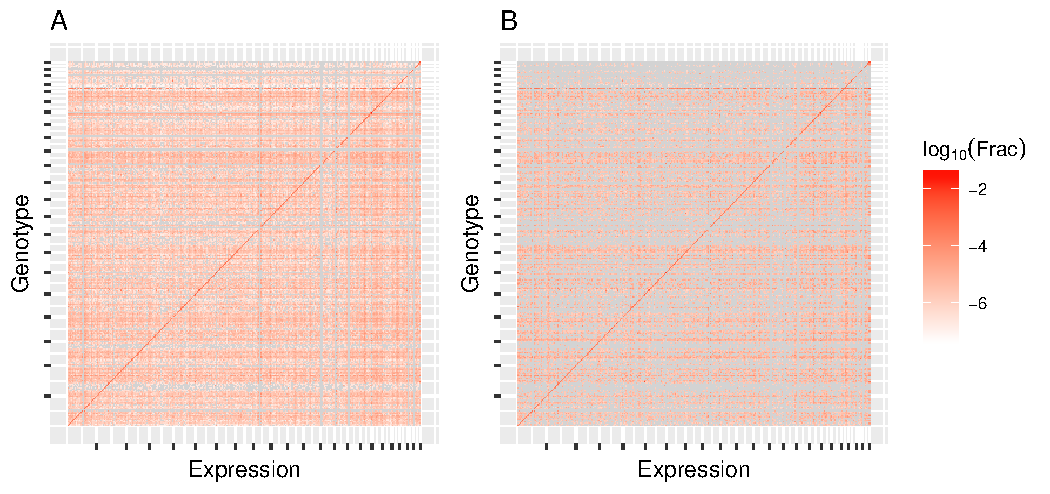
\includegraphics[scale = 1, keepaspectratio = true]{../figures/eqtl_all_herv_heatmap}  
	\caption{Fraction of SNP-expression probe pairs that were significantly associated sorted into bins according to their genomic locations. Ticks on the axis denote chromosome boundaries. Grey means there were no eQTMs in the given pair of bins. A considers all eQTLs an pairs, while B is limited on the ones whose SNP and/or expression probes are connected to HERV set 2.}
    \label{fig:global.eqtl.heatmap}
\end{figure}

A GO enrichment was performed on all 8211 genes associated to HERV related eQTLs using the set of all genes found in eQTLs as background. However, there were no significantly enriched genes. 

\subsection{eQTMs}
When calculating expression quantitative trait methylation there were a total of 13.88 millions CpG-expression probe pairs within a distance of 50 Kpb or less of each other. The number of potential trans-acting pairs equaled around 23.22 billions. 

Calculating eQTMs with a significance threshold of 10e-6 for cis resulted in 8187 significant associations ($fdr<1.7e-3$) consisting of 5957 distinct CpG sites and 1959 different expression probes. 1658 of these probes are annotated to 1461 genes, while there are no gene annotations for the remainder. 

361485 of the potential trans-action CpG-expression probe pairs proved to be significant at a p-value threshold of 10e-8 ($fdr<6.5e-4$). These trans-eQTLs are made up by 48206 CpGs and 11673 expression probes, for which 5738 gene annotations are available. 

The fractions of potential CpG-expression probe pairs that were significantly associated between their genomic locations are shown in figure \ref{fig:global.eqtm.heatmap}A. In contrast to the eQTL results there is only a weaker preference for cis interactions. 

HERV S2 contains 311 CpG sites and 420 expression probes, that were present in cis-eQTMs. A total of 738 cis-eQTMs are related to the set. 33 of these are associations between one of 33 CpG sites within a HERV element and one of 14 expression probes. 

Considering trans-eQTMs, 1109 significantly associated CpGs lie within HERV S2 and 5422 expression probes overlapping a HERV element are part of a trans-eQTM.

\begin{figure}[tb]
	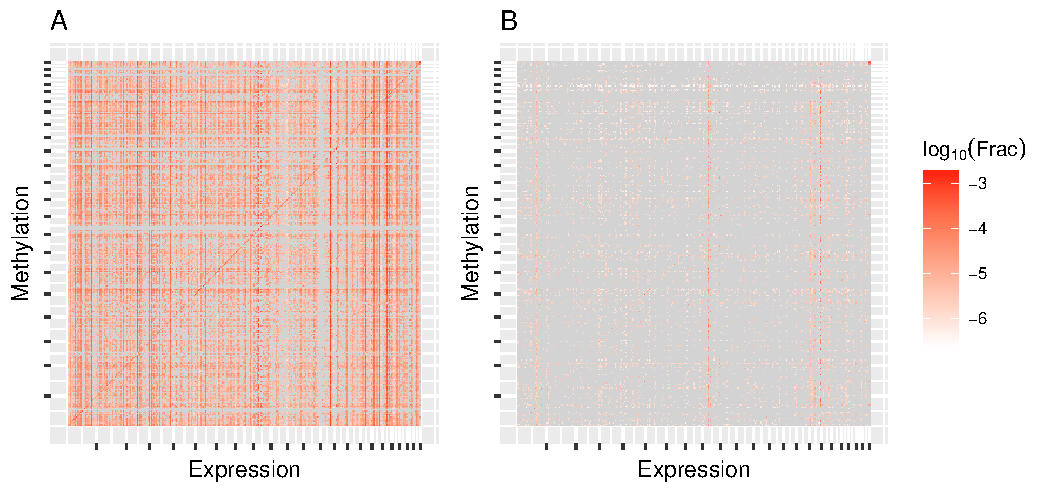
\includegraphics[scale = 1, keepaspectratio = true]{../figures/eqtm_all_herv_heatmap}  
	\caption{Fraction of CpG-expression probe pairs that were significantly associated sorted into bins according to their genomic locations. Ticks on the axis denote chromosome boundaries. Grey means there were no eQTMs in the given pair of bins. A considers all eQTLs an pairs, while B is limited on the ones whose SNP and/or expression probes are connected to HERV set 2.}
    \label{fig:global.eqtm.heatmap}
\end{figure}

The results of GO biological process enrichment performed on the xxxx genes that the expression probes found in HERV S2 related eQTMs are shown in table \ref{tab:hervS2.eqtm.enrichment}. 
%whatever is in that fricking table


\subsection{meQTLs}

\subsection{HERV related regulatory networks}
\subsubsection{Data collection}


\newpage
\section{Discussion}

\newpage
\section{Conclusion and Outlook}

\newpage
\bibliography{mybib}{}
\bibliographystyle{unsrt}

\end{document}